\chapter{Существующие алгоритмы} \label{ch:ch2}

\section{Анализ} \label{sec:ch2/sec1}

В основном в качестве источника информации используются статьи \cite{dai, hodge, vakili, varun, billor, wilkinson}. Помимо статей интерес представляют датасеты, которые тоже предстояло найти. Среди датасетов есть хорошо известный MNIST с набором изображений рукописных цифр, а также данные о разных сортах винных изделий, свободных электронах в ионосфере Земли, о заболеваниях сердца и другие. \cite{billor}

В этой работе рассматриваются стационарные данные. Поиск аномалий во временных рядах, а также прогнозирование временных рядов находятся за рамками рассматриваемой в работе темы.

\section{Основы алгоритмов} \label{sec:ch2/sec2}

Задачу поиска аномалий можно отнести к классу задач обучения без учителя. Суть поиска аномалий заключается в том, чтобы найти в выборке объекты, которые не похожи на большинство объектов выборки, т. е. те, которые выделяются на фоне других.

Часто бывает так, что аномальных объектов либо нет вообще, либо их очень мало и неизвестно где именно в выборке они находятся. Поэтому поиск аномалий относится к классу задач обучения без учителя (т. к. отсутствуют размеченные данные).

\subsection{Метрики}

\todo{Метрики типа ROC-AUC, Precision, Recall, etc.}



\section{Подходы к решению} \label{sec:ch2/sec3}

Одним из возможных способов определения аномалий является измерение схожести между объектов. У такого способа есть два варианта:
\begin{enumerate}
  \item Восстановление плотности
  \item Классификация
\end{enumerate}

\subsection{Восстановление плотности}

В случае с восстановлением плотности необходимо построить распределение, которое хорошо описывает выборку. И это распределение позволяет посчитать вероятность для нового объекта получить его из распределения, описывающего выборку.

В терминах этого метода аномалия - объект, полученный из другого распределения, описывающего другую выборку данных.

\noindent Есть три подхода:
\begin{enumerate}
  \item Параметрический
  \item Непараметрический
  \item Восстановление смесей
\end{enumerate}

\noindent\textbf{Параметрический метод}

Распределение представляется в виде $p(x)=\phi(x\vert\theta)$, где $\theta$ выступает в качестве параметра распределения. Например, в семейство параметрических распределений входит распределение Гаусса - $\theta=(\mu, \Sigma)$, где $\mu$ - вектор средних и $\Sigma$ - ковариационная матрица.

Параметры модели подбираются таким образом, чтобы вероятность объектов из обучающей выборки была максимальной. Для этого обычно пользуются Методом Максимального Правдоподобия:

\[ \sum_{i}\log\phi(x_{i}\vert\theta) \rightarrow \max_{\theta} \]

Есть ещё Автокодировщики, которые хорошо справляются с понижением размерности данных и с помощью которых можно хорошо семплировать из заданного распределения \cite{karazeev}.

\section{Алгоритмы} \label{sec:ch2/sec4}

\noindent В текущей работе были рассмотрены следующие алгоритмы:

\begin{enumerate}
	\item k-Nearest Neighbors (k-NN) \cite{knn} -- метод k-ближайших соседей.
	\item Principal Component Analysis (PCA) \cite{pca} -- метод главных компонент.
	\item One-Class Support Vector Machines (OCSVM) \cite{ocsvm} -- одноклассовый метод опорных векторов.
	\item Local Outlier Factor (LOF) \cite{lof} -- метод локального уровеня выброса.
	\item Histogram-Based Outlier Score (HBOS) \cite{hbos} -- оценка выбросов на основе гистограммы.
	\item Isolation Forest \cite{iforest} -- метод изолируещего леса.
	\item Single-Objective Generative Adversarial Active Learning (SO-GAAL) \cite{gaal} -- одно-объективное порождающее состязательное активное обучение.
\end{enumerate}

\section{Датасеты} \label{sec:ch2/sec5}

\noindent Для проверки сервиса были рассмотрены следующие датасеты:
\begin{enumerate}
  \item Arrhythmia -- определение наличия аритмии по данным ЭКГ \cite{guvenir}.
  \item Breast Cancer -- определение типа опухоли молочной железы: доброкачественная или злокачественная.
  \item Glass -- идентификация типа стекла, оставленного на месте преступления.
  \item Ionosphere -- рассматриваются характеристики радаров, которые используется в анализе ионосферы: необходимо определить является радар "плохим" или "хорошим".
  \item Letter Recognition -- по описанию изображения определить присутствует ли буква из английского алфавита или нет
  \item Mammography -- детектирование микрокальцинатов по данным маммографии
  \item MNIST -- научиться различать изображения рукописных цифр 6 и 0
  \item Satellite -- определение типа почвы по спутниковым снимкам.
\end{enumerate}
В качестве источника этих данных выступает библиотека ODDS \cite{odds}.

\begin{table} [htbp]
	\centering
	\caption{Статистика по данным из рассматриваемых датасетов}\label{tab:stats}%
	\begin{tabular}{lrrr}
		\toprule
		     Датасет & Кол-во объектов & Размерность &  Процент выбросов \\
		\midrule
		  arrhythmia &      452 &         274 &      14.60 \\
		     breastw &      683 &           9 &      34.99 \\
		       glass &      214 &           9 &       4.21 \\
		  ionosphere &      351 &          33 &      35.90 \\
		      letter &     1600 &          32 &       6.25 \\
		 mammography &    11183 &           6 &       2.33 \\
		       mnist &     7603 &         100 &       9.21 \\
		   satellite &     6435 &          36 &      31.64 \\
		\bottomrule
		\hline
	\end{tabular}
\end{table}

Сравнение данных, которые представлены в указанных датасетах.

\begin{figure}[ht]
  \centering
  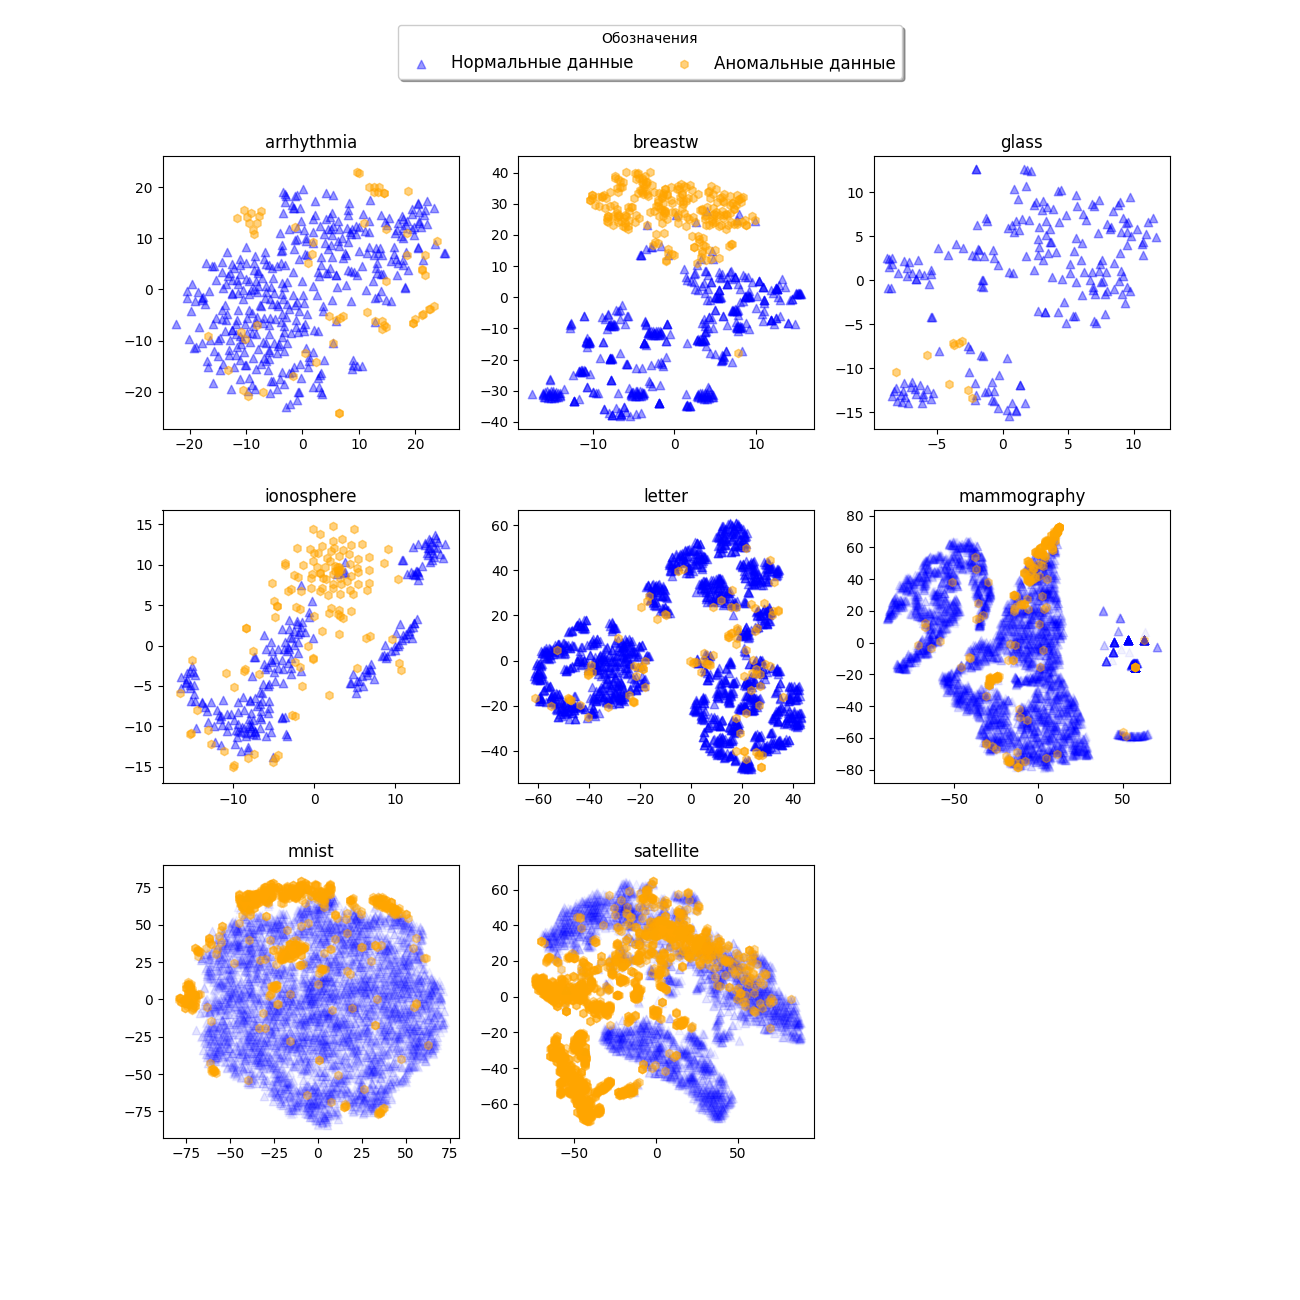
\includegraphics[width=\textwidth, height=\textheight, keepaspectratio] {2d_comparison}
  \caption{Рассматриваемые датасеты после применения алгоритма понижения размерности t-SNE}
  \label{fig:2d_comparison}
\end{figure}

\todo{Сравнение алгоритмов на датасетах}

\begin{table} [htbp]
	\centering
	\caption{Значения ROC для рассматриваемых алгоритмов на данных}\label{tab:rocs}%
	\begin{tabular}{lrrrrrr}
		\toprule
		     Датасет &   KNN &   PCA &  OCSVM &   LOF &  HBOS &  IFOREST \\
		\midrule   
   		arrhythmia &  0.7555 &  0.7794 &  0.7825 &  0.7672 &  0.7831 &   \textbf{0.7849} \\
     breastw &  \textbf{0.9908} &  0.9608 &  0.9649 &  0.4574 &  0.9764 &   0.9872 \\
       glass &  \textbf{0.8558} &  0.7308 &  0.8077 &  0.6538 &  0.7500 &   0.7212 \\
  ionosphere &  \textbf{0.9460} &  0.8115 &  0.8684 &  0.9023 &  0.6190 &   0.8632 \\
      letter &  \textbf{0.8660} &  0.5119 &  0.5985 &  0.8530 &  0.5532 &   0.5770 \\
 mammography &  0.8346 &  \textbf{0.9039} &  0.8911 &  0.6806 &  0.8506 &   0.8680 \\
       mnist &  0.8322 &  \textbf{0.8493} &  0.8487 &  0.6727 &  0.5607 &   0.7942 \\
   satellite &  0.6795 &  0.5601 &  0.6274 &  0.5567 &  \textbf{0.7464} &   0.7008 \\
		\bottomrule
		\hline
	\end{tabular}
\end{table}

\begin{figure}[ht]
  \centering
  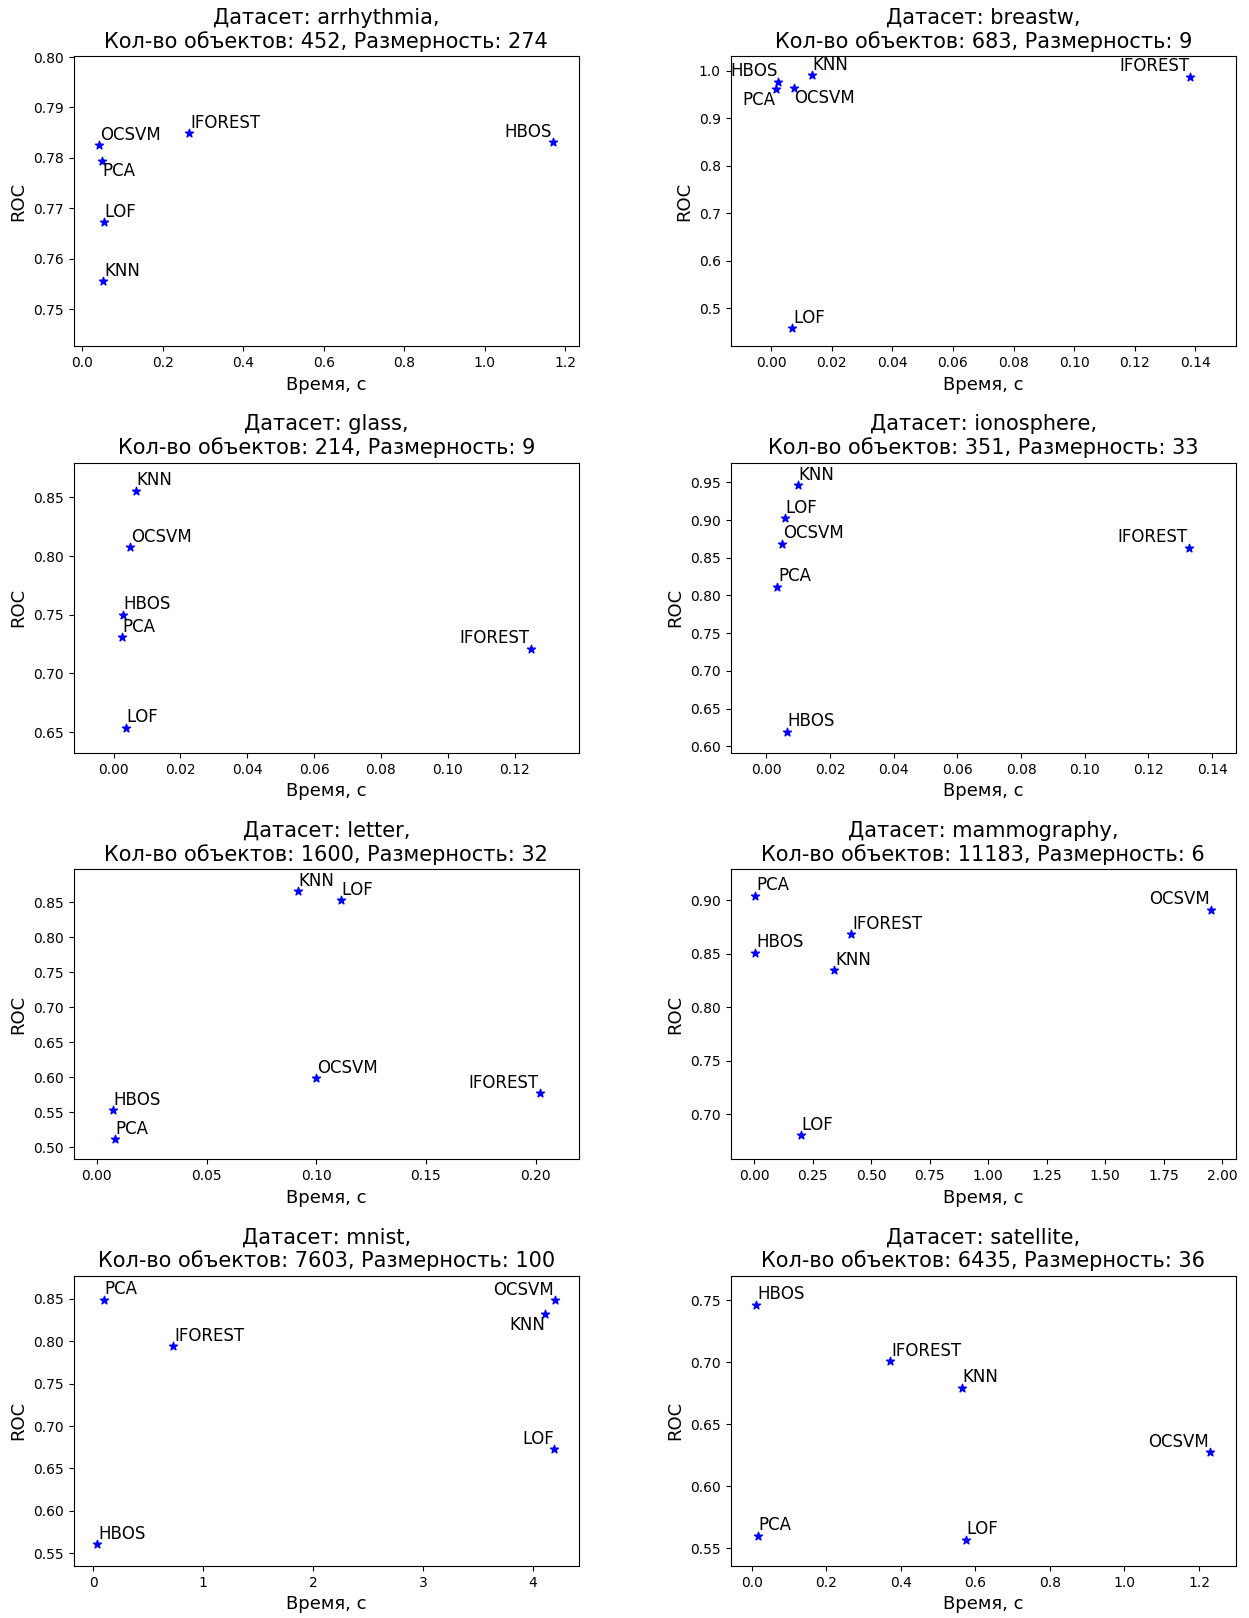
\includegraphics[width=\textwidth, height=\textheight, keepaspectratio] {roc_vs_time}
  \caption{Эффективность алгоритмов на разных датасетах}
  \label{fig:roc_vs_time}
\end{figure}

При построении графиков, которые изображены на рисунке~\ref{fig:roc_vs_time}, использовалась библиотека adjustText\footnote{\url{https://github.com/Phlya/adjustText/}}.

\begin{figure}[ht]
  \centering
  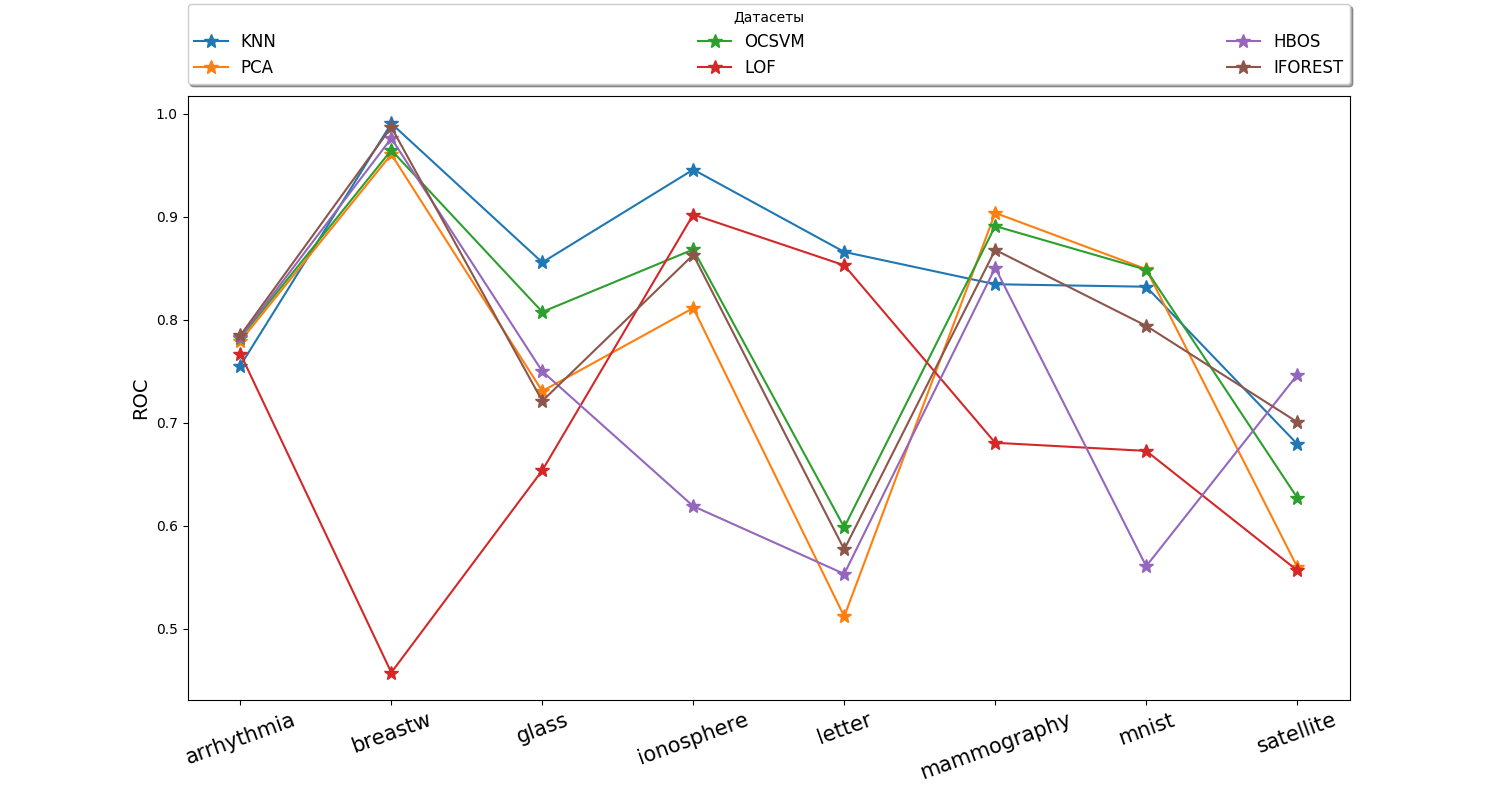
\includegraphics[width=\textwidth, height=\textheight, keepaspectratio] {roc_vs_dataset}
  \caption{Качество алгоритмов в зависимости от датасета}
  \label{fig:roc_vs_dataset}
\end{figure}

%\begin{figure}[ht]
%  \centering
%  
\includegraphics [scale=0.27] {latex}
%  \caption{TeX.}
%  \label{fig:latex}
%\end{figure}
%
%\section{Длинное название параграфа, в котором мы узнаём как сделать две картинки с~общим номером и названием} \label{sec:ch2/sect2}
%
%А это две картинки под общим номером и названием:
%\begin{figure}[ht]
%  \begin{minipage}[ht]{0.49\linewidth}\centering
%    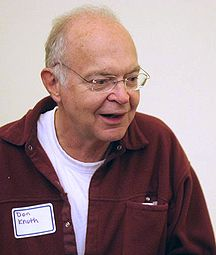
\includegraphics[width=0.5\linewidth]{knuth1} \\ а)
%  \end{minipage}
%  \hfill
%  \begin{minipage}[ht]{0.49\linewidth}\centering
%    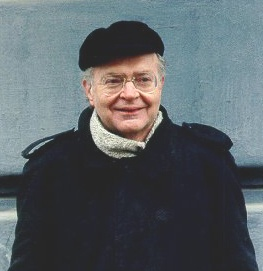
\includegraphics[width=0.5\linewidth]{knuth2} \\ б)
%  \end{minipage}
%  \caption{Очень длинная подпись к изображению,
%      на котором представлены две фотографии Дональда Кнута}
%  \label{fig:knuth}
%\end{figure}
%
%Те~же~две картинки под~общим номером и~названием,
%но с автоматизированной нумерацией подрисунков:
%\begin{figure}[ht]
%    {\centering
%        \hfill
%        \subbottom[List-of-Figures entry][Первый подрисунок\label{fig:knuth_2-1}]{%
%            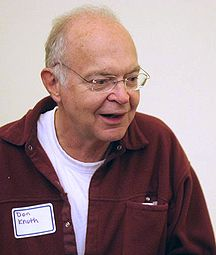
\includegraphics[width=0.25\linewidth]{knuth1}}
%        \hfill
%        \subbottom[\label{fig:knuth_2-2}]{%
%            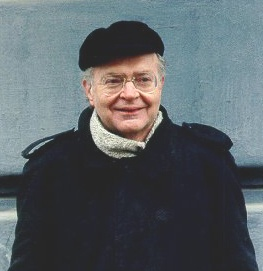
\includegraphics[width=0.25\linewidth]{knuth2}}
%        \hfill
%        \subbottom[Третий подрисунок]{%
%            \includegraphics[width=0.3\linewidth]{example-image-c}}
%        \hfill
%    }
%    \legend{Подрисуночный текст, описывающий обозначения, например. Согласно
%    ГОСТ 2.105, пункт 4.3.1, располагается перед наименованием рисунка.}
%    \caption[Этот текст попадает в названия рисунков в списке рисунков]{Очень
%    длинная подпись к второму изображению, на~котором представлены две
%    фотографии Дональда Кнута}
%    \label{fig:knuth_2}
%\end{figure}
%
%На рисунке~\ref{fig:knuth_2-1} показан Дональд Кнут без головного убора.
%На рисунке~\ref{fig:knuth_2}\subcaptionref*{fig:knuth_2-2}
%показан Дональд Кнут в головном уборе.